% INFORMS 2026 Data Mining Society Data Challenge — written report
% NOTE: all figures quoted here are regenerated by `python3 canonical.py` into
% CANONICAL.md. After the freeze rebuild, re-verify §6 against that file.
\documentclass[10pt,letterpaper,twocolumn]{article}
\usepackage[margin=0.72in]{geometry}
\usepackage{times}
\usepackage{amsmath,amssymb}
\usepackage{booktabs}
\usepackage{array}
\usepackage[normalem]{ulem}
\newcommand{\meth}[1]{\uline{#1}}   % the method terms, underlined in the abstract
\newcolumntype{L}[1]{>{\raggedright\arraybackslash}p{#1}}
\usepackage{graphicx}
\usepackage[table]{xcolor}
\usepackage[colorlinks=true,linkcolor=black,citecolor=black,urlcolor=black]{hyperref}
\usepackage{titlesec}
\usepackage{caption}
\usepackage{stfloats}                  % allow table*/figure* at the bottom in twocolumn
\setcounter{topnumber}{3}\setcounter{bottomnumber}{2}\setcounter{totalnumber}{4}
\renewcommand{\topfraction}{0.92}\renewcommand{\bottomfraction}{0.7}
\renewcommand{\textfraction}{0.06}\renewcommand{\floatpagefraction}{0.75}
\captionsetup{font=small,labelfont=bf,skip=3pt}
\titlespacing*{\section}{0pt}{6pt}{3pt}
\titlespacing*{\subsection}{0pt}{5pt}{2pt}
\titleformat{\section}{\normalfont\large\bfseries}{\thesection}{0.6em}{}
\titleformat{\subsection}{\normalfont\normalsize\bfseries}{\thesubsection}{0.6em}{}
\setlength{\abovedisplayskip}{4pt}
\setlength{\belowdisplayskip}{4pt}
\setlength{\parskip}{0pt}
\newcommand{\rmsev}[1]{\texttt{#1}}

\title{\vspace{-2.2em}\textbf{What Is Recoverable?}\\[2pt]
\large An Error-Budget Approach to County-Transfer\\Outage Forecasting}
\author{\normalsize\textbf{Team Bee2}\\[3pt]
\normalsize Hamed Khosravi (team leader) \qquad Melika Baghi\\[2pt]
\footnotesize INFORMS 2026 Data Mining Society Data Challenge}
\date{\vspace{-1em}}

\begin{document}
\maketitle
\vspace{-1.5em}

\begin{abstract}\small
\noindent We forecast hourly county Outage Severity Index (OSI) at four horizons
for 63 counties never seen in training, through a two-wave March 2026 wind event.
Rather than searching model space, we first measured \meth{how the residual error
decomposes}, because that determines where attention is worth spending. The
diagnosis --- computed before the later experiments, from cached out-of-fold
predictions and without retraining --- puts the error at roughly $45\%$ county
\meth{scale}, $37\%$ trajectory \meth{shape} and $17\%$ \meth{timing}, with no
dominant mode, and finds that whatever a model still gets wrong about a county's
overall magnitude is not recoverable from any legal feature we could construct
(out-of-fold $R^2\!\approx\!0$; $-0.09$ with 219 features and boosted trees).
That diagnosis was turned into falsifiable predictions for eight
\meth{intervention families}, and 210 controlled models plus a further 28 paired
contrasts were used to test them. The resulting forecaster is an equal-weight
$50/50$ blend of two halves --- eleven diverse models sharing one half, and a
single high-variance-reduction model holding the other --- with \meth{no
fitted combination parameters}, scoring \textbf{0.00838} (mean of the
four horizon RMSEs with the configuration choice itself nested; a reporting
summary, not the official ranking statistic) against $0.01632$ for
all-zeros and $0.01110$ for decayed persistence. The full ledger, the
code, and an interactive dashboard over all 210 models ship with this
submission; §\ref{sec:repro} says where.

\smallskip
\noindent\fbox{\parbox{0.955\linewidth}{The ensemble's most valuable members are
its \emph{worst} models: the three stock-flow models are the weakest of the
eleven and the three least correlated with the rest, and no substitute survived
a replacement test. Separately, the largest single improvement we made to a
member made the ensemble \emph{significantly worse} ($P{=}0.011$), and ten
further variance-reduction experiments reproduced that pattern. Both follow from one
property of a 239-county sample: a member's marginal value to the ensemble is
\textbf{not determined by its solo RMSE}, and residual complementarity can
dominate it.}}
\end{abstract}

\section{Task, protocol, and diagnosis}
\label{sec:diag}

\textbf{Task.} Each county has a 216-hour event window. Hours 0--71 are
observed for every county, test counties included; outage variables are withheld
from hour 72 onward. The submission is indexed by 144 origins per county
(hours 72--215) and four horizons, so the scored targets span hours 73--215 ---
143 distinct hours, since hour 72 is an origin but never a target. Weather is
given for all 216 hours, so the exogenous drivers are known across the forecast
window: the horizon is twice the context and the covariates carry the dominant
signal. Training and test counties are disjoint (239 / 63), so this is
\emph{cross-sectional} transfer --- the model sees a test county's first 72
hours but never its storm outcome, and no post-origin outage value is available
at inference. $42.4\%$ of scored cells are exactly zero and the target has skew
$8.8$.

\textbf{Metric.} RMSE is computed separately for each of four horizons
($t{+}1,6,24,48$\,h) over $9009/8694/7560/6048$ valid cells, and teams are
ranked \emph{within} each horizon with the four ranks averaged. There is no
official scalar; the mean of the four RMSEs used throughout this report is a
reporting convenience, and we verify that every design decision improves all
four horizons rather than only the mean.

\textbf{Protocol.} Table~\ref{tab:proto} is the whole of it. Every number in
this report was produced under it, unchanged, from the first model to the last;
nothing below is a figure we could have obtained by relaxing one of its rows.

\begin{table}[b]\footnotesize\centering
\setlength{\tabcolsep}{3.2pt}
\begin{tabular}{@{}L{1.42cm}L{3.10cm}L{3.72cm}@{}}
\toprule
& what we do & why it is the right choice here \\
\midrule
validation & five-fold cross-validation holding out \emph{counties}, stratified
  by state $\times$ severity &
  the scored set is 63 counties disjoint from training, so folds must withhold
  counties, not hours \\[2pt]
causality & every outage-derived column set to NaN after hour 71, \emph{before}
  features are built &
  validation and deployment share one code path; overwriting every post-origin
  outage value with garbage moves predictions by exactly $0.0$ \\[2pt]
nesting & anything learned across folds --- a scalar, a member set, a rule ---
  is fit on four folds and applied to the fifth &
  a choice made by looking at all five folds is itself a fitted
  parameter;
  Fig.~\ref{fig:conc} (right) shows what ignoring this costs \\[2pt]
testing & paired county bootstrap: resample the 239 counties with
  replacement, apply the \emph{same} resample to both models &
  pairing removes the county draw, which is far larger than any margin we
  test; we report the win fraction and a percentile interval \\[2pt]
statistic & per-horizon RMSE at $t{+}1,6,24,48$\,h; the mean of the four is a
  reporting convenience only &
  the official ranking is by average rank \emph{within} each horizon, so every
  decision is checked on all four columns \\
\bottomrule
\end{tabular}
\caption{The validation protocol, fixed before the experiments and never
varied. Four of the five rows cost us results we would otherwise have claimed.}
\label{tab:proto}
\end{table}

\textbf{Diagnosis.} Decomposing the residual of an early ensemble by substituting
each of a county's true scale, shape and timing in turn gives roughly
$45/37/17$, with no dominant mode. Two further measurements sharpen it. First,
the per-county residual multiplier --- what a model still gets wrong about a
county's overall magnitude --- is not predictable out of fold from any legal
feature set we built, including 219 aggregated features with boosted trees
($R^2 = -0.09$). Second, the error is spatially concentrated: 14 of 239 counties
carry $65\%$ of it, and $82\%$ of squared error is \emph{under}-prediction of
outages that did occur. Exact zeros, despite being $42.4\%$ of cells, carry
$0.7\%$.

\begin{figure*}[t]
\centering
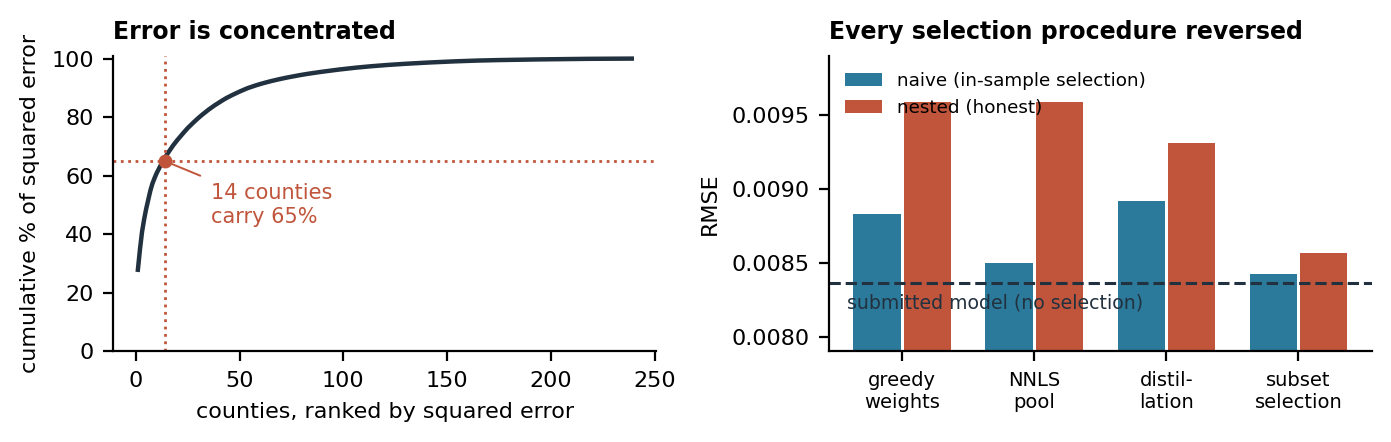
\includegraphics[width=\textwidth]{fig1_concentration_staircase.png}
\caption{Left: squared error against counties ranked by their contribution ---
14 counties carry $65\%$. Right: four selection procedures, scored naively and
with the selection itself nested inside the folds. Every one reverses.}
\label{fig:conc}
\end{figure*}

This is an empirical statement about what our features and learners recover, not
a proof of irreducibility. Read that way it still generates sharp predictions:
interventions that add information or change the function class should return
little, because the missing quantity is not in the features and is not a
function-class artefact; interventions that reduce estimator variance or make
models fail \emph{differently} should return more, because $191$ sequences per
fold is a small-sample regime. The rest of the paper tests those predictions.

\section{The intervention program}
\label{sec:ledger}

An experiment is classified by the \emph{contrast} it was run to test, not by
the properties of the model it produced. A shipped member may be a bi-GRU with a
dual objective and snapshot averaging; the experiment that admitted it changed exactly
one of those against a control. Eight mutually exclusive families exhaust our
experimental ledger:

\smallskip
\noindent\textbf{F1} signal $\cdot$ \textbf{F2} mechanism $\cdot$ \textbf{F3}
target $\cdot$ \textbf{F4} exposure $\cdot$ \textbf{F5} estimation $\cdot$
\textbf{F6} adaptation $\cdot$ \textbf{F7} combination $\cdot$ \textbf{F8}
uncertainty
\smallskip

\noindent plus two book-keeping codes: \textbf{P} for procedures whose object is
choosing or evaluating rather than predicting, and \textbf{X} for models that
deliberately changed more than one stage and so cannot serve as clean evidence
for either.

What makes the eight mutually exclusive is that they are the \emph{stages of a
single pipeline}, in order: Table~\ref{tab:sep} names the stage each one owns.
A model may of course combine several previously accepted changes --- most of
the shipped ones do --- but the family records the one contrast that admitted
it, so no model is counted twice. Table~\ref{tab:fam} is the record;
\texttt{family\_ledger.py} regenerates it from the experiment log. Four
families --- F1, F2, F5 and F6 --- had the \emph{direction} of their outcome
written down before the corresponding models existed; the rest complete the
ledger.

\begin{table}[t]\footnotesize\centering
\setlength{\tabcolsep}{3.4pt}
\begin{tabular}{@{}l L{1.60cm} L{2.06cm} L{1.98cm}@{}}
\toprule
& stage it changes & the question it asks & an example contrast \\
\midrule
\textbf{F1} & what goes in & does more information help? & $+$ external statics \\
\textbf{F2} & how inputs map to outputs & does another function class help? & GRU $\to$ PatchTST \\
\textbf{F3} & what is predicted & does another target scale help? & $y \to \sqrt{y}$ \\
\textbf{F4} & what it trains on & does perturbing exposure help? & $+$ storm jitter \\
\textbf{F5} & how it is estimated & does less estimator variance help? & 1 seed $\to$ 25 \\
\textbf{F6} & what happens afterwards & does correcting the output help? & isotonic recalibration \\
\textbf{F7} & how models are pooled & does another combination rule help? & mean $\to$ amp.$\times$shape \\
\textbf{F8} & what is claimed & does the stated interval cover? & split conformal \\
\bottomrule
\end{tabular}
\caption{The eight families are the eight stages of one forecasting pipeline,
which is what makes them mutually exclusive: a controlled experiment changes
exactly one stage and holds the other seven fixed. This is why an experiment is
classified by its \emph{contrast} and not by the model it produced.}
\label{tab:sep}
\end{table}

\begin{figure*}[b]
\centering
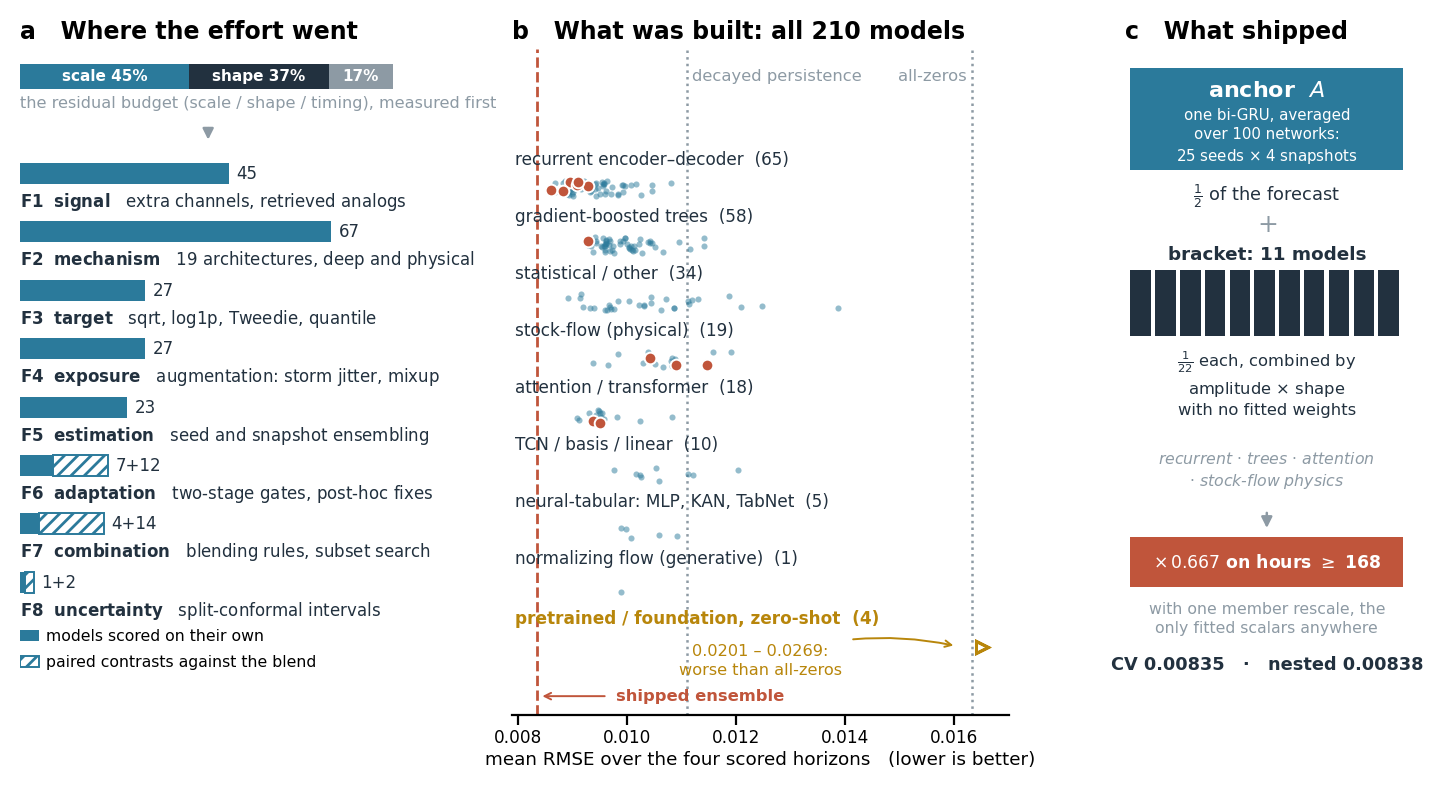
\includegraphics[width=\textwidth]{fig4_procedure.png}
\caption{The whole procedure. \textbf{(a)} A residual budget measured before any
model existed allocated attention across eight families; solid bars are models
scored on their own, hatched bars are paired contrasts against the blend.
\textbf{(b)} All 210 models, by class and by score under the single protocol of
Table~\ref{tab:proto}; the twelve that shipped are ringed. Only the four
pretrained forecasters fall off the axis --- they lose to predicting zero
everywhere. \textbf{(c)} What survived: one heavily averaged anchor holding half
the forecast, eleven dissimilar models sharing the other half, one quiet-tail
scalar, and no fitted combination weight anywhere.}
\label{fig:proc}
\end{figure*}


\begin{table*}[!t]\small\centering
\begin{tabular}{@{}llccL{4.55cm}L{5.25cm}@{}}
\toprule
& family & models & paired & diagnostic implication & what the contrasts showed \\
& & scored & contrasts & & \\
\midrule
F1 & signal & 45 & 0 & the residual is unrecoverable from the feature sets tested; with 191 sequences/fold, extra channels should have small or negative marginal value in high-capacity models &
  external statics and sub-county weather help the tabular member; the same channels \emph{lose} in 3/3 sequence models, which is the capacity asymmetry the hypothesis predicts; retrieved analogs fail \\
F2 & mechanism & 67 & 0 & error is spread across scale, shape and timing, so no function-class substitution should unlock a step change &
  5 of 6 architecture families land at or behind a plain GRU; Chronos-2 zero-shot scores worse than predicting zero; a mediocre patch transformer is retained only because it fails differently \\
F3 & target & 27 & 0 & $42.4\%$ zeros are cheap ($0.7\%$ of squared error); skew is expensive &
  $\sqrt{y}$-target beats raw by $6\%$ and beats log1p; the dual raw$/\sqrt{y}$ objective and metric-aligned hour weights transfer; Tweedie, quantile, hurdle and a likelihood-trained flow all lose on RMSE \\
F4 & exposure & 27 & 0 & robust perturbation can manufacture distinct error bases &
  storm jitter and mixup survive as distinct bases; multi-origin and dropout variants do not \\
F5 & estimation & 23 & 0 & 191 sequences/fold implies variance-limited estimators &
  seed and snapshot averaging improve nearly every model \emph{alone}; ten of ten fail to improve the blend \\
F6 & adaptation & 7 & 12 & the per-county residual has out-of-fold $R^2\!\approx\!0$, so post-hoc correction should fail &
  0 of 12 corrections help: isotonic, power-law, per-hour curves, severity multipliers, and both the zero gate and the county gate. Only a mechanism-backed quiet-tail scalar survives \\
F7 & combination & 4 & 14 & with no dominant error mode, complementary residuals should matter &
  fitted weights, NNLS, distillation and subset selection all reverse under nesting; a parameter-free amplitude$\times$shape rule wins \\
F8 & uncertainty & 1 & 2 & orthogonal to the point metric &
  split-conformal intervals reach $0.900$ coverage at every horizon and leave RMSE unchanged \\
\midrule
P & protocol & 4 & 0 & \emph{book-keeping, not a hypothesis} & Ray and Optuna searches; tuned configurations do not beat the untuned control \\
X & compound & 5 & 0 & \emph{book-keeping, not a hypothesis} & changed two stages at once; kept in the ledger, excluded from family evidence \\
\midrule
& \textbf{total} & \textbf{210} & \textbf{28} & & \\
\bottomrule
\end{tabular}
\caption{The experimental ledger; nine further attempts crashed on a code fault
without producing output and are excluded. \emph{Models scored} each have their
own out-of-fold score. \emph{Paired contrasts} are tests of a change measured
against the shipped ensemble rather than on its own --- a combination rule or a
post-hoc correction has no solo score to report, so it can only be evaluated
this way; a $0$ means the family contains no such test, not a missing entry.
F1, F2, F5 and F6 had their direction recorded before those models existed.}
\label{tab:fam}
\end{table*}

\textbf{F2, in detail, because it is the family most readers expect to pay.}
Nineteen architectures were run on this protocol, each adapted to consume the
known-future weather so that none was tested where it is weakest. The
2023--2026 exogenous-covariate family lands at $0.0095$--$0.0120$
(PatchTST~\cite{nie} $0.0095$, TSMixer~\cite{tsmixer} $0.0098$,
iTransformer~\cite{liu} $0.0102$, TimeXer~\cite{timexer} $0.0108$,
XLinear $0.0111$, DLinear $0.0120$) against $0.0088$--$0.0090$ for the recurrent
members. Only one architecture outside the recurrent family earned a seat, and
not for its accuracy.

\textbf{Foundation models, measured rather than dismissed.} The obvious modern
move is a pretrained forecaster --- a family whose usefulness for forecasting
has been questioned on other benchmarks~\cite{tan} --- and the obvious objection --- that these models
assume univariate input with no known future --- stopped being true with the
covariate-aware generation, so we ran one. \textbf{Chronos-2}~\cite{chronos2} (120M) scores
$0.0213$ zero-shot given our 23 weather covariates and $0.0201$ without them:
both \emph{worse than predicting zero everywhere} $(0.0163)$, and the covariates
make it worse rather than better. The failure is diagnosable --- it places
non-zero mass almost everywhere, $3.2\%$ exact zeros against $42.4\%$ in the
truth, so it cannot represent a target silent on nearly half its cells. Four
tabular foundation models (TabPFN, TabDPT, TabICLv2, Mitra) were prepared as
drop-in learners for the tabular member on its exact rows; two are gated behind
a licence or a GPU, and the rest were stopped once the sequence result made the
outcome clear. None is shippable regardless: a checkpoint pretrained on outside
corpora is external data of a kind the self-contained-code requirement does not
admit. We report the number because ``foundation models do not transfer here''
is worth more as a measurement than as an assertion.

\textbf{F3, in detail, because skew dominates the target.} With $42.4\%$ zeros
and skew $8.8$, squared error on the raw scale is set by a handful of
county-hours. Fitting on $\sqrt{\mathrm{OSI}}$ and inverting improves the same
gradient-boosted model from $0.01028$ to $0.00967$; log1p over-corrects
($0.00996$). But squaring a $\sqrt{y}$-scale fit back is biased by Jensen's
inequality, and RMSE rewards the conditional mean: the tabular member predicts
$0.841$ of the truth on average. The members that matter therefore use a
\emph{dual} objective, half the error on each scale, which buys the variance
stabilisation without the back-transform bias. Removing the bias entirely from
the tabular member --- Duan's smearing estimator, ratio $0.841 \to 1.01$ ---
improves that member alone and makes the ensemble \emph{worse}; the partial
rescale that all five folds adopt leaves it shrunk. The blend wants that member
biased low, which is the shrinkage result of §\ref{sec:diag} arriving from a
second direction.

The same family covers the probabilistic objectives. A conditional normalizing
flow trained by maximum likelihood, with its sample mean as the point forecast,
reaches $0.0099$ --- respectable, and not admitted, because RMSE rewards the
conditional mean and an MSE-trained network estimates it directly rather than
through sampling. Tweedie and quantile heads behave the same way: better models
of the distribution, worse answers to the question asked.

\textbf{Two-stage and hurdle models, tested three ways and rejected.} The
obvious reading of $42\%$ zeros is a two-part model, and it is what the
operational outage literature, dominated by tree ensembles on storm-level
exposure features, reaches for. A perfect zero classifier would move the score
by $0.00003$, because those cells carry $0.7\%$ of the error. Measured, as a target
factorisation: $P(y{>}0) \times E[y\,|\,y{>}0]$, fitted separately on the
tabular member's rows, is worse on all four horizons than the single-stage
model, because training the magnitude head on positives alone discards what the
zeros say about magnitude. The corresponding \emph{post-hoc} versions --- a
boosted classifier gating the finished ensemble, and a random-forest gate
splitting counties before choosing a configuration per group --- are F6 and fail
there: the county gate is worse by $0.0004$, and still worse by $0.00003$ when
its gate is replaced by the true grouping. The zeros are also not a phase: counties show a median of four separate zero runs, and 178 of 239 are
already non-zero at the origin, so there is no onset to predict.

\section{The forecaster the evidence leaves}
\label{sec:model}

Three families shaped the final model: F4 created alternative error bases, F5
reduced estimator variance where that gain outweighed the diversity it costs,
and F7 exploited what complementarity remained. What survives is an equal-weight
blend of two objects,
\[
\hat{y} \;=\; \tfrac{1}{2}\,\mathcal{C}\big[f_1,\dots,f_{11}\big]
\;+\; \tfrac{1}{2}\,A ,
\]
followed by the quiet-tail scalar. Twelve trained predictors go into the
forecast, in two unequal halves.

The \textbf{bracket} $\mathcal{C}[f_1,\dots,f_{11}]$ is eleven diverse models
sharing half the weight, so each carries $1/22$ of the forecast. $\mathcal{C}$
combines them by \emph{amplitude and shape separately} --- the mean of their
per-county totals times the mean of their normalised trajectories. It is
parameter-free, equals the plain mean when the members agree on timing, and
preserves peak height when they do not, because averaging in raw space spends
amplitude to hedge timing disagreement.

The \textbf{anchor} $A$ is one model holding the other half by itself. It is the
same bi-directional GRU as two of the bracket members, but estimated $25$ seeds
$\times$ 4 cosine-restart snapshots --- $100$ networks averaged --- which makes
it the most accurate single object in the project at $0.00862$ and by far the
lowest-variance. It is called the anchor because that is its job: it holds the
forecast steady while the bracket supplies disagreement. It sits outside the
bracket rather than inside it for a measured reason. Placed as a twelfth member
it would receive $1/12$ of the weight, and a paired county bootstrap says that
under-weights it --- it is as good alone as the whole eleven-member bracket, and
the $50/50$ split is the only fixed weighting that says so. That split is
\emph{not} fitted: $1/2$ and $1/11$ are the two round numbers the structure
implies, and §\ref{sec:model} shows what happened every time we tried to fit
them instead.

\begin{table}[ht]\small\centering
\begin{tabular}{@{}llcc@{}}
\toprule
member & mechanism / admitting contrast & alone & corr \\
\midrule
$A$ & recurrent; F5 schedule diversity & 0.00862 & --- \\
\midrule
\texttt{x9} & recurrent; F5 snapshots & 0.00884 & 0.84 \\
\texttt{s62} & recurrent; F3 hour weights & 0.00897 & 0.81 \\
\texttt{i11w} & recurrent; F4 storm jitter & 0.00909 & 0.79 \\
\texttt{x4} & recurrent; F4 mixup & 0.00912 & 0.82 \\
\texttt{s35w} & recurrent; F3 on the mixup base & 0.00930 & 0.80 \\
\texttt{f2} & trees; F1 external statics & 0.00930 & 0.83 \\
\texttt{s39} & attention; F1 other counties & 0.00939 & 0.82 \\
\texttt{ts2c} & patch transformer; F2 & 0.00952 & 0.79 \\
\texttt{p1b} & stock-flow; F2 & 0.01042 & 0.78 \\
\texttt{r6corr} & stock-flow; F6 flow scalars & 0.01090 & 0.73 \\
\texttt{p1c} & stock-flow; F4 teacher-forced & 0.01148 & 0.70 \\
\bottomrule
\end{tabular}
\caption{The anchor $A$ --- one model holding half the forecast --- and the
eleven bracket members sharing the other half, each labelled by the family of
the contrast that admitted it.
Shipped members inherit earlier accepted interventions; the label is the
\emph{provenance}, not a claim that they differ in one respect only.}
\label{tab:mem}
\end{table}

\begin{figure}[t]
\centering
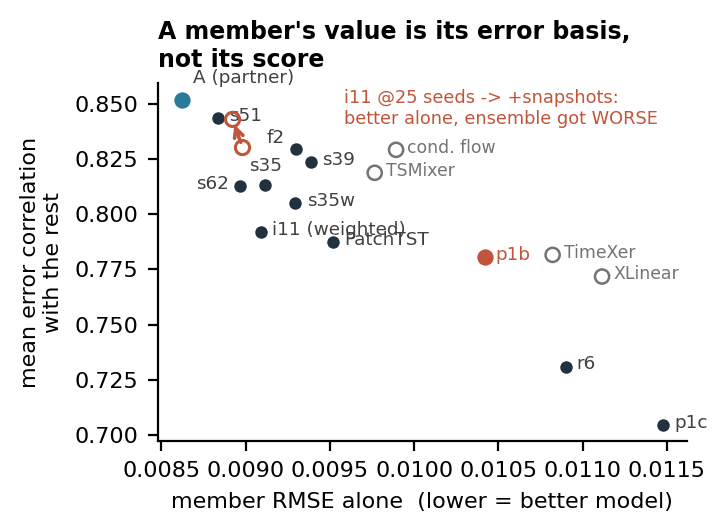
\includegraphics[width=\linewidth]{fig3_diversity.png}
\caption{Each object by how good it is alone (horizontal) against how much its
errors resemble the rest (vertical). The useful direction is \emph{down}, not
left. The three stock-flow models are the worst in the set and the only ones far
from the crowd. The arrow shows a member being genuinely improved: it moves left
and also up, and the ensemble got worse.}
\label{fig:div}
\end{figure}

\textbf{The worst member is the one to keep.} \texttt{p1b} is barely better than
decayed persistence and ranked first of 28 candidates for its seat; every
attempt to replace it made the blend worse at all four horizons. Two further
stock-flow variants were admitted later by an add-one sweep over every cached
object, and they are the two least correlated members in the set. Doubling the
existing physics weight does \emph{not} help, so these are new bases rather than
more of the same one.

\textbf{Improving a member can cost more than it buys.} Snapshot-ensembling one
member improved it from $0.00955$ to $0.00892$ --- its best score ever --- and
made the ensemble significantly worse ($P{=}0.011$), because the technique drove
its errors onto $A$'s, and $A$ is itself a snapshot ensemble. Re-running all ten
remaining members at 25 seeds turned that anecdote into a controlled sweep: six
of the ten improved \emph{alone} --- one by $0.00031$ --- two got worse because
they already average internally, and the two tree-based members were unchanged
because their seed only moves subsampling. Not one was adopted into the blend on
a single fold, and all ten together scored $0.00848$ against $0.00835$. Variance
reduction is the family with the best solo returns and the worst ensemble
returns, and the two facts have the same cause.

\textbf{Nothing in the combination is fitted.} Every weight above is fixed in
advance. Fitting the full simplex buys $0.000007$, while greedy weights, NNLS
pooling, distillation and exhaustive subset selection all reverse under nesting
(Fig.~\ref{fig:conc}, right) --- five folds returned five different answers each
time. Exactly two fitted scalars survive anywhere in the model, both nested and
both mechanism-backed: the quiet-tail factor, and the tabular rescale of
§\ref{sec:ledger}.

\section{Results and uncertainty}
\label{sec:results}

\begin{center}\small
\begin{tabular}{@{}lccccc@{}}
\toprule
model & $t{+}1$ & $t{+}6$ & $t{+}24$ & $t{+}48$ & mean \\
\midrule
all-zeros & 23.49 & 19.82 & 12.09 & 9.87 & 16.32 \\
decayed persistence & 12.79 & 11.92 & 10.19 & 9.49 & 11.10 \\
best single model ($A$) & 10.16 & 9.23 & 7.90 & 7.20 & 8.62 \\
\textbf{submitted ensemble} & \textbf{9.94} & \textbf{9.07} & \textbf{7.57} & \textbf{6.83} & \textbf{8.35} \\
\bottomrule
\end{tabular}
\end{center}
\vspace{-2pt}
{\footnotesize RMSE $\times 10^{3}$. The four horizon columns are what the
organisers score; \emph{mean} is our reporting summary. The horizons are not
comparable to each other --- $t{+}48$ scores only hours $120$--$215$, after the
second wave, where the target is smaller and more often zero --- but they are
comparable across teams, which is how the ranking works.}

The ensemble improves on the strongest naive baseline by $25\%$ and removes
$73\%$ of the target's squared magnitude, against $54\%$ for persistence. It is
better than the eight-member predecessor at all four horizons. Two figures
should be distinguished: $0.00835$ is the out-of-fold score of the fixed final
configuration, and $\mathbf{0.00838}$ is the estimate when the choice among the
ten configurations searched is itself nested inside the folds. The second is the
honest one and is what we quote wherever a single number carries the claim; the
$0.00003$ between them is what the selection is worth, and reporting only the
first is the mistake the right-hand panel of Fig.~\ref{fig:conc} is about.
Figure~\ref{fig:traj} shows forecasts for four held-out counties.

\textbf{Where the blend earns its keep.} Hours $72$--$95$ carry $51\%$ of all
squared error, and there the eleven-member blend scores $0.01777$ against
$0.01778$ for $A$ alone: it contributes nothing. From hour 96 onward it beats
decayed persistence by $20$--$39\%$. The reason is visible in the same window:
on the 24 counties holding $84.5\%$ of early error, the model's correlation with
truth is $0.887$ and its bias is $0.887$ --- the shape is right and the level is
$11\%$ low. Every member makes that same error, so there is no disagreement for
a blend to exploit. Diversity pays only where members genuinely differ. This
also explains why severity-targeted corrections fail: severity itself \emph{is}
predictable --- the ensemble's own county totals rank it at AUC $0.985$ --- but
the counties we get \emph{wrong} overlap the most severe ones only 6 of 13, and
a multiplier keyed on the best available severity ranking is worse on all four
horizons out of fold.

\textbf{Conformal intervals.} A point forecast with no statement of its own
uncertainty is a weak deliverable for an operational task, so we calibrated
split-conformal intervals on four folds and checked them on the fifth. Coverage
is $0.900$ at every horizon against a nominal $90\%$, and scaling the conformity
score by the prediction gives locally adaptive intervals $22$--$48\%$ narrower
at the same coverage --- which matters, because interval width varies by two
orders of magnitude across counties. Two caveats we state rather than hide:
cells within a county are not exchangeable, so this is a county-split check and
not a formal guarantee; and the point forecast is unchanged by construction, so
none of it moves the RMSE we are scored on. Interval calibration and point
accuracy are separable here, and conformal prediction is why we can say so.

\textbf{We do not claim separation from comparable submissions.} Resampling 63
counties gives a score standard deviation of $0.0016$: roughly $45\times$ the
margin between our final model and our own earlier ones, larger than the entire
spread of the 2025 finalist field, and enough to move our own score between
$0.0055$ and $0.0114$. Any ranking at the fifth decimal is substantially a
statement about which counties were held out.

\begin{figure*}[t]
\centering
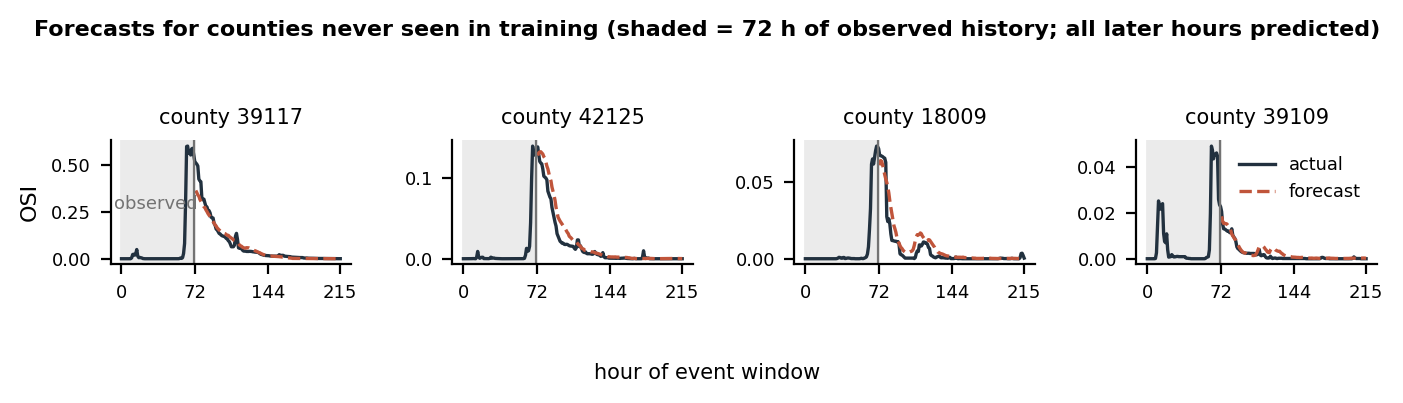
\includegraphics[width=\textwidth]{fig2_trajectories.png}
\caption{Forecasts for four counties never seen in training, spanning the
severity range. Shaded: the 72 observed hours. Everything after is predicted.}
\label{fig:traj}
\end{figure*}

\section{Conclusion and reproducibility}
\label{sec:repro}

A pre-experiment residual diagnosis allocated attention across a closed set of
intervention families; $210$ controlled models and $28$ paired contrasts then
tested those family-level predictions under county-held-out, nested validation.
The model emerged from the interventions that survived, not from ranking
configurations. The finding we would carry to another problem is that in a
small-sample transfer regime a component's marginal value is governed by the
complementarity of its errors at least as much as by their size --- which is why
the three weakest models in our set are the three we could not remove.

\textbf{Limits.} The residual result is empirical, not information-theoretic:
the per-county multiplier is unrecoverable by the features and learners we
tested, not unpredictable in principle. One member consumes external static
data; a package-only substitute costs $0.00004$, measured, and ships as a
one-line fallback. All numbers are county-holdout estimates on the 239 training
counties, not leaderboard scores.

\texttt{make\_submission.py} rebuilds the prediction file end-to-end from the
three provided CSVs with fixed seeds and no manual steps; a clean clone
reproduces a byte-identical SHA-256. \texttt{canonical.py} regenerates every
number quoted here from cached out-of-fold predictions, so any citation can be
checked by re-running rather than by trusting. All of it is submitted as
\texttt{code.zip}, self-contained and needing no network access.

{\footnotesize An interactive dashboard over all 210 models --- every one
sortable, the members plotted by accuracy against error correlation, and a
builder that returns the exact held-out score of any subset of 60 you combine
--- ships inside \texttt{code.zip} as \texttt{catalogue/dashboard.html}, a
single self-contained file that opens from disk with no server and no network,
so nothing below is needed to read it. \meth{The same code and the full
catalogue in four formats are also at}
\textbf{\url{https://github.com/HamedKhosravi99/informs2026-model-catalogue}},
\meth{with the dashboard served at}
\textbf{\url{https://hamedkhosravi99.github.io/informs2026-dashboard/}}.
\textbf{Both are private while the competition is open and become public on
25 September 2026}, once the deadline has passed, so the committee can inspect
them directly --- and \textbf{we are glad to open either sooner on request} if
that suits the review schedule.}

{\footnotesize
\begin{thebibliography}{9}\small
\bibitem{nie} Y.~Nie et al. A time series is worth 64 words: long-term
forecasting with transformers. \emph{ICLR}, 2023.
\bibitem{liu} Y.~Liu et al. iTransformer: inverted transformers are effective
for time series forecasting. \emph{ICLR}, 2024.
\bibitem{tan} M.~Tan et al. Are language models actually useful for time series
forecasting? \emph{NeurIPS}, 2024.
\bibitem{timexer} Y.~Wang et al. TimeXer. \emph{NeurIPS}, 2024.
\bibitem{tsmixer} S.-A. Chen et al. TSMixer. \emph{TMLR}, 2023.
\bibitem{chronos2} A.~F. Ansari et al. Chronos-2. arXiv:2510.15821, 2025.
\end{thebibliography}}

\end{document}
